\chapter{Wymagania funkcjonalne}
\label{Chapter3}

Wymagania funkcjonalne (ang. functional requirements) określają co system powinien oferować użytkownikowi, to jest jakie operacje można na nim wykonać. Ważne jest, by utrzymać kompletny zbiór poprawnie zdefiniowanych wymagań, pomaga to w zrozumieniu w jaki sposób powinien działać system, nawet dla osób które nie mają wiedzy technicznej oraz pomaga podczas jego projektowania.

Niniejszy rozdział przedstawia wymagania funkcjonalne za pomocą dwóch najpopularniejszych sposobów ich opisu, są to: przypadki użycia (ang. use cases)  oraz opowieści użytkownika (ang. user stories). Pierwsza z metod polega na określeniu listy kroków. Reprezentuje ona interakcję między aktorem a systemem. Wykonanie kroków skutkuje osiągnięciem celu, który ma zapewnić system. Druga metoda - Opowieści użytkownika przedstawia w kilku zdaniach potrzebę użytkownika, którą ma realizować system. 

\begin{figure}[th] 
\centering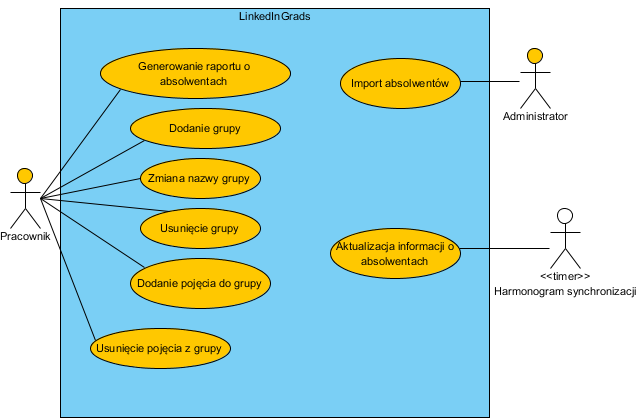
\includegraphics[width=15cm]{figures/image1}
\caption{Diagram przypadków użycia}\label{rys:use-case-diagram}
\end{figure}

\subsection{Generowanie raportu o absolwentach}

\ucsection{UC1: Generowanie raportu o absolwentach}{Pracownik dziekanatu, System}
{}
{}{\ucactions{
\ucaction{1. Pracownik wybiera opcję generowania raportu.}
\ucaction{2. System prezentuje typy raportów do wyboru.}
\ucaction{3. Pracownik wybiera typ raportu.}
\ucaction{4. System prezentuje rok ukończenia studiów do wyboru.}
\ucaction{5. Pracownik wybiera rok ukończenia studiów.}
\ucaction{6. Pracownik inicjuje generowanie raportu.}
\ucaction{7. System prosi o wybranie ścieżki zapisu raportu.}
\ucaction{8. Pracownik wybiera ścieżkę zapisu.}
}}
{}

\subsection{Dodanie grupy}

\ucsection{UC2: Dodanie grupy}{Pracownik dziekanatu, System}
{}
{}{\ucactions{
\ucaction{1. Pracownik wybiera opcję dodania grupy.}
\ucaction{2. System prosi o podanie nazwy grupy.}
\ucaction{3. Pracownik podaje nazwę grupy.}
\ucaction{4. System informuje o pomyślnym dodaniu grupy.}
}}
{\ucextensions{
\ucaction{3.A. Grupa o podanej nazwie już istnieje.}
\ucaction{3.A.1. System informuje o błędzie.}
\ucaction{3.A.2. Powrót do kroku 3.}
}}
{}

\subsection{Zmiana nazwy grupy}

\ucsection{UC3: Zmiana nazwy grupy}{Pracownik dziekanatu, System}
{}
{}{\ucactions{
\ucaction{1. Pracownik wybiera opcję zmiany nazwy grupy.}
\ucaction{2. System prezentuje listę istniejących grup.}
\ucaction{3. Pracownik wybiera grupę.}
\ucaction{4. System prosi o podanie nowej nazwy grupy.}
\ucaction{5. Pracownik podaje nową nazwę grupy.}
\ucaction{6. System informuje o pomyślnej zmianie nazwy grupy.}
}}
{\ucextensions{
\ucaction{5.A. Grupa o podanej nazwie już istnieje.}
\ucaction{5.A.1. System informuje o błędzie.}
\ucaction{5.A.2. Powrót do kroku 3.}
}}
{}

\subsection{Usunięcie grupy}

\ucsection{UC4: Usunięcie grupy}{Pracownik dziekanatu, System}
{}
{}{\ucactions{
\ucaction{1. Pracownik wybiera opcję usunięcia grupy.}
\ucaction{2. System prezentuje listę istniejących grup.}
\ucaction{3. Pracownik wybiera grupę do usunięcia.}
\ucaction{4. System informuje o pomyślnym usunięciu grupy.}
}}
{}

\subsection{Dodanie pojęcia do grupy}

\ucsection{UC5: Dodanie pojęcia do grupy}{Pracownik dziekanatu, System}
{}
{}{\ucactions{
\ucaction{1. Pracownik wybiera opcję grupowania pojęć.}
\ucaction{2. System prezentuje listę istniejących grup.}
\ucaction{3. Pracownik wybiera grupę.}
\ucaction{4. System prezentuje listę pojęć niezgrupowanych.}
\ucaction{5. Pracownik wybiera pojęcie do dodania.}
\ucaction{6. System informuje o pomyślnym dodaniu pojęcia do grupy.}
}}
{\ucextensions{
\ucaction{3.A. Grupa została w międzyczasie usunięta.}
\ucaction{3.A.1. System informuje o błędzie.}
\ucaction{3.A.2. Powrót do kroku 2.}
\ucaction{5.A. Grupa została w międzyczasie usunięta.}
\ucaction{5.A.1. System informuje o błędzie.}
\ucaction{5.A.2. Powrót do kroku 2.}
}}
{}

\subsection{Usunięcie pojęcia z grupy}

\ucsection{UC6: Usunięcie pojęcia z grupy}{Pracownik dziekanatu, System}
{}
{}{\ucactions{
\ucaction{1. Pracownik wybiera opcję grupowania pojęć.}
\ucaction{2. System prezentuje listę istniejących grup.}
\ucaction{3. Pracownik wybiera grupę.}
\ucaction{4. System prezentuje listę pojęć przypisanych do grupy.}
\ucaction{5. Pracownik wybiera pojęcie do usunięcia.}
\ucaction{6. System informuje o pomyślnym usunięciu pojęcia z grupy.}
}}
{\ucextensions{
\ucaction{3.A. Grupa została w międzyczasie usunięta.}
\ucaction{3.A.1. System informuje o błędzie.}
\ucaction{3.A.2. Powrót do kroku 2.}
}}
{}

\subsection{Aktualizacja informacji o absolwentach}

	\begin{tabular}{| p{.9\textwidth} |}
		\hline
		\textbf{Opowieść użytkownika:} US1 \\
		\hline
		\textbf{Opis:} Przebieg aktualizacji informacji o absolwentach. Odbywa się automatycznie, w tle działającego systemu. \\
		\hline
		\textbf{Treść:} Jako Pracownik chcę aby System, co ustalony czas pobierał informacje o absolwentach z portalu LinkedIn, a
następnie aktualizował swoją bazę danych. \\
		\hline  
	\end{tabular}
	
\subsection{Import absolwentów}

\ucsection{UC7: Import absolwentów}{Administrator, System}
{}
{}{\ucactions{
\ucaction{1. Pracownik wywołuje skrypt importu absolwentów.}
\ucaction{2. System prezentuje listę dodanych absolwentów.}
}}
{\ucextensions{
\ucaction{1.A. Niepoprawne dane wejściowe.}
\ucaction{1.A.1. System przerywa import i informuje o błędzie.}
\ucaction{1.A.2. Powrót do 1.}
}}
{}	

\subsection{Grupowanie pojęć}

	\begin{tabular}{| p{.9\textwidth} |}
		\hline
		\textbf{Opowieść użytkownika:} US2 \\
		\hline
		\textbf{Opis:} Generowanie raportu z użyciem mechanizmu grupowania pojęć. \\
		\hline
		\textbf{Treść:} Jako Pracownik chcę aby pojęcia (umiejętności, stanowiska, organizacje) w wygenerowanym raporcie były
pogrupowane (np. za pomocą metody LDA) w bardziej ogólne zbiory. 
 \\
		\hline  
	\end{tabular}